\documentclass[a4paper, 11pt, titlepage]{article}
\usepackage{fancyhdr}
\usepackage{graphicx}
\usepackage{imakeidx}
\usepackage{makeidx}
\usepackage{mathtools}
\usepackage[spanish]{babel}
\usepackage{eurosym}
\usepackage{hyperref}
\usepackage{amssymb}
\usepackage{listings}
\usepackage{xcolor}

\setcounter{secnumdepth}{5}
\setcounter{tocdepth}{5}

\title{\textbf{Software de gestión de información confidencial basado en Python}\\ 
Trabajo Fin de Grado Superior en Desarrollo de Aplicaciones Multiplataforma}
\author{Francisco Javier Balón Aguilar}
\date{21 de junio de 2018}

\begin{document}

\maketitle
\renewcommand{\contentsname}{Índice}
\tableofcontents
\newpage

\section{Estudio preliminar del problema}

    El presente documento detalla la el desarrollo del proyecto denominado Securebox, 
    realizado como proyecto integrado para la obtención del título de Técnico en 
    Desarrollo de Aplicaciones Multiplataforma por parte del centro Grupo Studium, 
    Sevilla. 

    El objetivo del proyecto consiste en desarrollar un software multiplataforma que 
    permita la gestión y almacenamiento de información, garantizando principalmente 
    la confidencialidad y la integridad de la información utilizando criptografía. 

    El software desarrollado soportará la gestión de usuarios, pudiendo existir 
    varios usuarios en la misma base de datos, siendo cada uno de ellos propietario 
    de diferentes secretos. 

    \subsection{Funciones básicas}

        \subsubsection{Control de acceso}

            El software almacena usuarios y contraseñas para realizar su función. 
            Es una función indispensable en el sistema, ya que cada fichero e 
            información irá vinculada directamente al usuario. Securebox es multiusuario, 
            en un equipo podrá haber varios usuarios pero sólo uno mantendrá una sesión 
            iniciada. A su vez, el sistema permite la creación de usuarios.

        \subsubsection{Gestión de información secreta}

            El núcleo lógico de Securebox es la gestión de información secreta. Esta 
            se almacenará en la base de datos junto a diferentes metadatos que permitan 
            el correcto desempeño de la aplicación. Podemos clasificar la información 
            secreta en archivos binarios y cadenas de texto.

            Los archivos binarios son ficheros de cualquier tipo y extensión. Pueden 
            ser imágenes, documentos, ficheros de texto, audio, vídeo, etc. Estos se 
            almacenarán en el sistema.

            Al igual que los archivos, las cadenas de texto permiten la gestión de 
            información introducida directamente por parte del usuario iniciado, de 
            forma que pueda almacenar de forma segura mensajes secretos, contraseñas, 
            pins, etc. Que serán almacenados en la base de datos.

    \subsection{Viabilidad del sistema}

        El lenguaje de programación orientado a objetos Python, utilizado como base 
        del sistema, crece en cuota de mercado a gran velocidad (véase figura \ref{py01}). 
        Estimándose como uno de los lenguajes más utilizados en el futuro próximo de la 
        tecnología (véase figura \ref{py02}), lo que 
        asegura un continuo soporte y comunidad. Estos factores favorecen un amplio 
        periodo en la línea temporal en el que esta aplicación podrá ser utilizada sin 
        quedar obsoleta, algo a tener en cuenta en un mundo tecnológico tan mutable.

        \begin{figure}[htp]
            \centering
            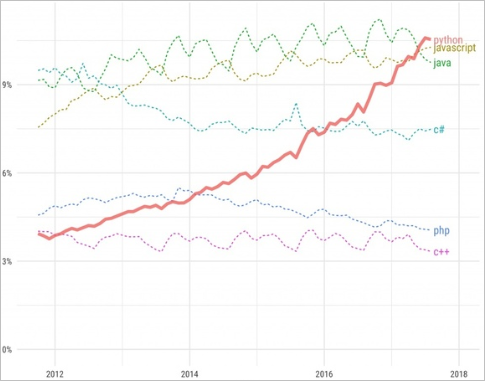
\includegraphics[width=0.7\textwidth]{resources/py01.png}
            \caption{Crecimiento de cuota de mercado del lenguaje Python.}
            \label{py01}
        \end{figure}

        Python se encuentra, de hecho, en uso constante en aplicaciones para la 
        ciberseguridad, tratamiento de datos masivos, implementando con grandes 
        resultado en el análisis de Big Data y minería de datos, programación científica 
        y data science y, últimamente, implementando materia de IA (Inteligencia 
        Artificial), Machine Learning, Deep Learning, etc.

        \begin{figure}[htp]
            \centering
            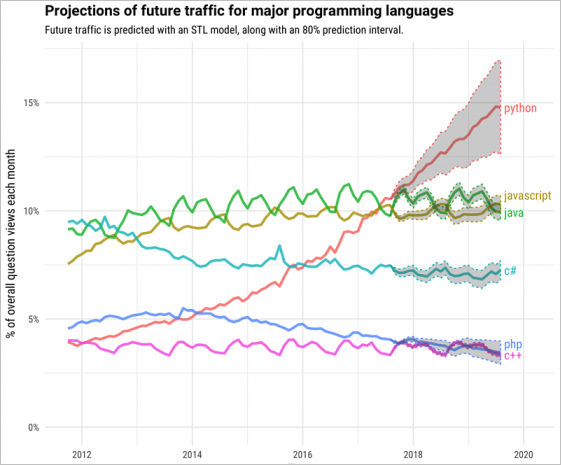
\includegraphics[width=0.7\textwidth]{resources/py02.png}
            \caption{Proyección de futuro del lenguaje Python.}
            \label{py02}
        \end{figure}
    
        Para situar al lector, podemos observar aplicaciones conocidas que implementan, 
        de una forma u otra, el lenguaje de programación Python; empresas y 
        organizaciones científicas con tan amplio volumen y flujos de información como 
        NASA, Nmag Computational Micromagnetic, National Geographic; grandes periódicos 
        y mass media como The Washington Post, The New York Time o grandes redes sociales 
        con miles de millones de usuarios como Instagram y Pinterest.

        Además, la planificación de aplicaciones aplicadas a la seguridad de la 
        información no deja de incrementarse en el tiempo; debido en gran parte a 
        los numerosos escándalos de graves fallos de seguridad, filtraciones de datos 
        sensibles, espionaje informático, el crecimiento del malware, estafas online, 
        etc. La sociedad, hoy, tiene más conciencia de protección de su información 
        cuando trabaja con tecnologías informáticas.

        Por estas razones, podemos concluir que, tras el análisis de viabilidad del proyecto, 
        este cumple las condiciones para considerarse viable y robusto en cuanto a su desarrollo 
        y mantenimiento en el tiempo.

\end{document}